\documentclass[9pt]{beamer}
\usepackage[spanish]{babel}
\usepackage[utf8]{inputenc}
\usepackage{multirow}
\usepackage{amsmath}
\usepackage{booktabs,calc,multirow}
\usepackage{amsfonts}
\usepackage{amssymb}
\usepackage{graphicx}
\usepackage{subcaption}
\usepackage{lipsum}
\usepackage{cases}
\usepackage{ragged2e}
\usepackage{tikz}
\usepackage{hyperref}
\usepackage{comment}
\usepackage{mathtools}
\usepackage{braket}
\usepackage{float}
\usepackage{url}
\usepackage{animate}
\usepackage{xcolor}
\definecolor{colorUva}{RGB}{0,107,166}
\definecolor{darkgreen}{rgb}{0.01, 0.25, 0.04}
\usetheme{Madrid}
\setbeamercolor{section in toc}{fg=black}
\setbeamercolor{subsection in toc}{fg=red}


\beamertemplatenavigationsymbolsempty
\title[ Transformadas Supersimétricas de Sistemas Cuánticos Unidimensionales.]{TESIS DOCTORAL EN FÍSICA:\\[0.1cm]Transformadas Supersimétricas de Sistemas Cuánticos Unidimensionales.}

\author[C. San Millán ]{Autor: Carlos San Millán Carpintero\\[0.2cm] Director: Manuel Gadella Urquiza}
\date{  
	12 de abril de 2024} 

\institute[UVa]{Departamento de Física Teórica, Óptica y Atómica, Universidad de Valladolid.}
\setbeamertemplate{background}{
\includegraphics[width=\paperwidth,height=\paperheight]{Fondo1.pdf}}
\date{12 de abril de 2024}
\setbeamertemplate{footline}{
  \leavevmode%
\hbox{%
	\begin{beamercolorbox}[wd=.20\paperwidth,ht=2.25ex,dp=1ex,center]{author in head/foot}%
		\usebeamerfont{author in head/foot}\insertshortauthor\hspace*{1em}
	\end{beamercolorbox}%
	\begin{beamercolorbox}[wd=.6\paperwidth,ht=2.25ex,dp=1ex,center]{title in head/foot}%
		\usebeamerfont{title in head/foot}\insertshorttitle\hspace*{1em}
	\end{beamercolorbox}%
	\begin{beamercolorbox}[wd=.2\paperwidth,ht=2.25ex,dp=1ex,right]{date in head/foot}%
		\usebeamerfont{date in head/foot}\insertsectionhead\hfill\insertframenumber{} / \inserttotalframenumber\hspace*{1ex}
\end{beamercolorbox}}%
\vskip0pt%
}


\begin{document}
	
	\begin{frame}
		\maketitle
		\vspace*{3 cm}
		\begin{tikzpicture}[remember picture, overlay]
			% Logo en la esquina superior izquierda
			%\node [anchor=south west,xshift=0.5 cm, yshift=1 cm] at (current page.south west) {\includegraphics[width=3cm]{resilencia.eps}};%
				\node [anchor=south west,yshift=0.2 cm] at (current page.south west) {\includegraphics[width=12.8 cm]{Capa 3.png}};
			\node [anchor=center,xshift=6.4cm, yshift=2.6 cm] at (current page.south west) {\includegraphics[width=3cm]{universidad-valladolid.eps}};
			% Logo en la esquina superior derecha
		%	\node [anchor=south east, yshift=0.7 cm] at (current page.south east) {\includegraphics[width=4cm]{qcayle.png}};%
			
		\end{tikzpicture}
		
	\end{frame}

	\begin{frame}{Introducción}
	La realización de esta Tesis Doctoral ha dado como resultado las siguientes publicaciones en revistas indexadas en el Journal Citation Reports (JCR): \vspace{1 cm}
	\begin{block}{}	\begin{itemize}
			\uncover<2->{\item  $[1]$ M. Gadella,  J. Hernández-Muñoz, L.M. Nieto y \alert<2>{C. San Millán}, "Supersymmetric Partners of the One-Dimensional Infinite Square Well Hamiltonian". \textit{Symmetry} , \textbf{13}, 350, (2021).} \vspace{0.5 cm}
		\uncover<3->{	\item  $[2]$ M. Gadella y \alert<3>{C. San Millán}, "Supersymmetric Partners of the One-Dimensional Infinite Square Well Hamiltonian: Special Cases".\textit{Symmetry}, \textbf{14}, 1314, (2022). } \vspace{0.5 cm}
		\uncover<4->{	\item $[3]$  \alert<4>{C. San Millán}, M. Gadella, Ş. Kuru y J. Negro," SUSY partners and S-matrix poles of the one-dimensional Rosen–Morse II potential". \textit{Eur. Phys. J. Plus } \textbf{138}, 857 (2023) }
	\end{itemize}\end{block}
\end{frame}


\begin{frame}{Índice}
	\tableofcontents
\end{frame}

\section[Capítulo 1]{Capítulo 1: Fundamentos Teóricos}
\begin{frame}{Capítulo 1: Fundamentos Teóricos}
	\tableofcontents[currentsection]
\end{frame}

\begin{frame}{Resonancias}
	\begin{block}{}
	 Sea un potencial \alert<1>{$V(x)$}, se busca la solución a la \alert<2>{E.S. } con energía positiva \alert<2>{ $E=k^2$}: 
	\begin{equation*}
	H \Psi(x)=k^2 \Psi(x)\, \quad \Psi(x)=A \alert<3>{ \phi(x)}+B\alert<3>{ \psi(x)}.
\end{equation*}
	\end{block}


	\uncover<4->{
		\begin{block}{}	
			\alert<4>{Matriz de transmisión}:
			\begin{equation*}
				\begin{pmatrix}
					\textcolor{magenta}{C} \\  \textcolor{blue}{D}
				\end{pmatrix}= \alert<4>{T(k)}	\begin{pmatrix}
					A \\  B
				\end{pmatrix}=	\begin{pmatrix}
					T_{11} & T_{12}\\  T_{21} & T_{22}
				\end{pmatrix} 	\begin{pmatrix}
					\textcolor{red}{A} \\  \textcolor{teal}{B}
				\end{pmatrix}
			\end{equation*}
		\end{block}
		
		\begin{block}{}
			\only<1-3>{\vspace{0.8\textheight}}
		\only<4,5>{	\begin{figure}
				\centering
				\animategraphics[autoplay,loop,width=0.8\textheight]{5}{gifS1/gifS1-}{1}{31}		
			\end{figure}
		}
		\end{block}
	}

	
	
\end{frame}
\begin{frame}{ Resonancias}
	\begin{block}{}
		\alert<2>{	Matriz $S$}:
				
				\begin{equation*}
					\begin{pmatrix}
						B \\ D
					\end{pmatrix}= \alert<2>{S}(k)	\begin{pmatrix}
						A \\  C
					\end{pmatrix}=\alert<3>{\frac{1}{T_{22}}}	\begin{pmatrix}
						-T_{21}&1\\  \det T& T_{12}
					\end{pmatrix} 	\begin{pmatrix}
						A \\  C
					\end{pmatrix}
				\end{equation*}
				Los estados confinados serán aquellos para los cuales las amplitudes de salida del potencial son infinitamente mayores que las de entrada:
				
	\end{block}
	\begin{block}{}

	\begin{figure}
				\centering
				\animategraphics[autoplay,width=0.8\textheight]{3}{gifS2/gifS2-}{1}{121}
			\end{figure}
	
			\end{block}



\end{frame}
\begin{frame}{Clasificación de los estados}
	
	{\setbeamercovered{transparent=100}
	\begin{block}{}
		\alert<1>{	\begin{equation}
				T_{22}(k)=0.\label{polo}
		\end{equation}}
		En función de la posición en $\mathbb{C}$ de $k$ que es raíz de la ecuación \eqref{polo} se pueden tener cuatro tipos de polo, que dan lugar a cuatro tipos de estado:
	\end{block}
		{\setbeamercovered{transparent=0}	\begin{block}{}\begin{itemize}
				\uncover<2->{	\item \textcolor{red}{Estados ligados}: Funciones de onda de cuadrado integrable, $k$ está en el semi-eje positivo imaginario.} \\[0.5cm] 
				\uncover<3->{\item \textcolor{blue}{Estados anti-ligados}: Funciones de onda que no son cuadrado integrable y divergen por los extremos,  $k$ está en el semi-eje negativo imaginario. }	\\[0.5cm]
				\uncover<4->{\item \textcolor{darkgreen}{Estados redundantes}: Aunque localizados en el eje semi-eje positivo imaginario, no son ligados, ya que no dan lugar a estados de cuadrado integrable. }
				\end{itemize}
	\end{block}		}
}
\end{frame}

	\begin{frame}{Mecánica Cuántica Supersimétrica }
	
		\begin{center}
			\begin{minipage}{0.6\textwidth}
				\begin{block}{Hamiltoniano inicial $H^{(0)}$}
					\begin{itemize}
											\item Autofunciones:  \alert<1>{$\phi^{(0)}_n$} y \alert<1>{$\psi^{(0)}_n$}
						\item Autovalores:  \alert<1>{$E^{(0)}_n$}
						
					\end{itemize}  
				\end{block}
			\end{minipage}
			
			
		\end{center}
		
	
				\begin{block}{}
					SUSY-QM: Relación entre dos hamiltonianos:
					\begin{equation}
						\alert<2>{H^{(0)}}=-\frac{d^2}{dx^2}+V^{(0)}(x),\quad \alert<2>{H^{(1)}}=-\frac{d^2}{dx^2}+V^{(1)}(x).
					\end{equation}
					
				\end{block}
				\vspace{-0.2 cm}
	\begin{block}{}
			\alert<3>{	Álgebra de operadores:}
					
					\begin{equation}
						A^\dagger H^{(0)}=H ^{(1)}A^\dagger, \quad 	A H^{(1)}=H ^{(0)}A,
					\end{equation}
			\end{block}
		
		\begin{block}{}
					Los hamiltonianos se expresan mediante \alert<4>{factorización}:
					\begin{equation}
						H^{(0)}=AA^\dagger,\quad H^{(1)}=A^\dagger A.
					\end{equation}
					
			\end{block}
			
		\end{frame}
		\begin{frame}{Mecánica Cuántica Supersimétrica }
					\begin{block}{}
						\alert<2>{Operadores de intercambio: $A$, y $A^\dagger$} :
						\begin{equation}
							A^\dagger=-\frac{d}{dx}+\alert<3>{W(x)},\quad A=\frac{d}{dx}+\alert<3>{W(x)}.
				\end{equation}\end{block}
			
			\begin{block}{}
					\alert<3>{	Superpotencial: $W(x)$ }
						\begin{equation}
						\alert<3>{W(x)}=-\frac{d}{dx}\log \alert<4>{\phi^{(0)}_\varepsilon}
						\end{equation}
				\end{block}
			\begin{alertblock}{Función semilla}
					\centering
					$\phi^{(0)}_\varepsilon(x)$ puede ser cualquier autofunción de $H^{(0)}$
				\end{alertblock}
			
			\end{frame}
	\begin{frame}{Mecánica Cuántica Supersimétrica }
	
	
	\begin{block}{}
				El potencial de $H^{(1)}$ viene dado por:
				\begin{equation}
					\alert<2>{V^{(1)}(x)}=V^{(0)}(x)-2\frac{d^2}{dx^2}\log \phi^{(0)}_\varepsilon(x)
				\end{equation}
		\end{block}
	\begin{block}{}
			Y sus funciones de onda por:
			\begin{equation}
			\alert<3>{	\phi_n^{(1)}(x)}=A^\dagger \phi_n^{(0)}(x)=\frac{\mathcal{W}( \phi_\varepsilon^{(0)}(x),\phi_n^{(0)}(x))}{\phi_\varepsilon^{(0)}(x)}
			\end{equation}
	\end{block}
\uncover<4->{	\begin{center}\begin{minipage}{0.6\textwidth}

			\begin{alertblock}{Espectro de $H^{(1)}$}
			$H^{(0)}$ y $H^{(1)}$ tienen el \alert<4>{mismo espectro}, excepto por un \alert<5>{número finito} de niveles.
		\end{alertblock}

\end{minipage}	\end{center}
\begin{block}{}\alert<6>{Potenciales invariantes de forma}: Aquellos a los que una transformada solo modifica sus parámetros pero no su dependencia funcional.
\end{block}}
	\end{frame}

	\begin{frame}{SUSY como simetría}
		\begin{block}{}
				Se define un \alert<1>{hamiltoniano matricial} y dos operadores matriciales (\alert<1>{supercargas}).
				\begin{equation}
					\alert<1>{\mathcal{H}}=\{Q^\dagger,Q\}=\operatorname{diag}\left(H^{(0)},H^{(1)}\right),
				\end{equation}
	\begin{equation*}
		\alert<1>{ Q^\dagger}=\frac{1}{2}(\sigma_1+i\sigma_2)A^\dagger,\quad \alert<1>{Q}=\frac{1}{2}(\sigma_1-i\sigma_2)A.
	\end{equation*}
		\end{block}
		\uncover<3->{		\begin{minipage}{0.45\linewidth}
		\begin{block}{	\alert<4-6>{SUSY es una simetría}}
			\begin{equation*}
			\alert<4>{	\bra{0}\mathcal{H}\ket{0}=0\equiv [Q,\mathcal{H}]=0}
			\end{equation*}
					\begin{itemize}
			\item	\alert<5>{E.F.  en $H^{(0)}$}, y $A^\dagger \phi^{(0)}_0=0,$
			\item \alert<6>{E.F.  en $H^{(1)}$}, y $A \phi^{(1)}_0=0.$
					\end{itemize}
			\end{block}
		\end{minipage}\hfill
		\begin{minipage}{0.45\linewidth}
			\begin{block}{\alert<7-10>{SUSY está rota}}
							\begin{equation*}
						\alert<8>{	\bra{0}\mathcal{H}\ket{0}\neq0\equiv [Q,\mathcal{H}]\neq0}
						\end{equation*}
					\centering \begin{itemize}
			\item  E.F.  de $\mathcal{H}$ \alert<9>{no nulo}
			\item Ambos hamiltonianos tienen el \alert<10>{mismo número de niveles}.
					\end{itemize}
			\end{block}
		\end{minipage}}
		
		
	
	\end{frame}
	
	\begin{frame}{SUSY de tipo I}

			\begin{center}
					\begin{minipage}{0.7\textwidth}
					{	\setbeamercolor{block title}{bg=white,fg=black}	\begin{block}{}
							\begin{figure}
								\centering
								\includegraphics[width=0.9\textwidth]{SUSY1.pdf}
							\end{figure}
					\end{block}}
	
			\begin{block}{SUSY de tipo I}
				\begin{itemize}
					\item 	\alert<2>{La semilla es el fundamental}
					\item \alert<3>{$H^{(1)}$ tiene un estado ligado menos}
					
				\end{itemize}
		\end{block}

		
					
						\end{minipage}
				
			\end{center}

		
			\end{frame}		
			
			\begin{frame}{SUSY de tipo II}
	
			
				\begin{center}
				\begin{minipage}{0.7\textwidth}
					{	\setbeamercolor{block title}{bg=white,fg=black}	\begin{block}{}
							\begin{figure}
								\centering
								\includegraphics[width=0.9\textwidth]{SUSY2.pdf}
							\end{figure}
					\end{block}}
					
					
				\only<3,4>{	\begin{block}{SUSY de tipo II}
							\begin{itemize}
								\item$H^{(1)}$ tiene  \alert<3>{un nivel más que}  $H^{(0)}$.
								\item $\phi_{\varepsilon}^{(0)}$  no es de cuadrado integrable.
								
							\end{itemize}
					\end{block}}

		
	
	\end{minipage}
					\only<1,2>{
					\begin{block}{SUSY de tipo II}
					
						\begin{equation}
						\alert<2>{	\phi^{(1)}_0(x)=\frac{1}{\phi_\varepsilon^{(0)}}},\quad 	\psi^{(1)}_0(x)=\frac{1}{\phi_\varepsilon^{(0)}}\int^{x}(\phi_\varepsilon^{(0)}(x'))^2 dx'
						\end{equation}
				\end{block}}			
			\end{center}
		\end{frame}
	
	\begin{frame}{SUSY rota}

		
		\begin{center}
			\begin{minipage}{0.7\textwidth}
				{	\setbeamercolor{block title}{bg=white,fg=black}	\begin{block}{}
						\begin{figure}
							\centering
							\includegraphics[width=0.9\textwidth]{NOSUSY.pdf}
						\end{figure}
				\end{block}}
				
				
			\begin{block}{SUSY  rota}
							\begin{itemize}
								\item $\phi_{\varepsilon}^{(0)}$  y  $1/\phi_{\varepsilon}^{(0)}$ \alert<4>{no son} de cuadrado integrable.
								\item $H^{(1)}$ tiene la \alert<3>{misma cantidad de estados ligados} que  $H^{(0)}$
								
								
							\end{itemize}
					\end{block}
						
					
				
			\end{minipage}
			
		\end{center}
	
			
	
	\end{frame}

	
	\begin{frame}{SUSY de orden $\ell$}


\begin{columns}

		\begin{column}{0.5\textwidth}
			{	\setbeamercolor{block title}{bg=white,fg=black}
			\begin{block}{}
				\begin{figure}
					\centering
					\includegraphics[width=1\textwidth]{nSUSYB.pdf}
					
				\end{figure}
		\end{block}}
	\end{column}\hfill
		\begin{column}{0.45\textwidth}
		\begin{block}{$H^{(\ell)}$ se describe mediante:}
			\begin{equation*}
			\alert<2>{	\phi^{(\ell)}_n}=B^\dagger\phi^{(0)}_n=\frac{\mathcal{W}(\{\phi_i^{(0)}\}_{i=0}^{\ell-1}\cup\{\phi_n^{(0)}\})}{\alert<3>{\mathcal{W}(\{\phi_i^{(0)}\}_{i=0}^{\ell-1})}},
			\end{equation*}
			\begin{equation*}
				\alert<4>{V^{(\ell)}}=V^{(0)}-2\partial_x^2\log \alert<4>{\mathcal{W}(\{\phi_i^{(0)}\}_{i=0}^{\ell-1})}
			\end{equation*}
		\end{block}
			\uncover<5->{	\begin{block}{Descomposición del operador}
				\begin{equation*}
					B^\dagger \propto A^{(1)}\dots A^{(\ell)}
				\end{equation*}	\end{block}}
	\end{column}
\end{columns}
		
\uncover<6->{\begin{center}
		\begin{minipage}{0.7\textwidth}
			\begin{alertblock}{Transformada ordinaria}
				Aquella que elimina niveles en orden \alert<7>{ascendiente de energía}, partiendo del \alert<7>{fundamental}.
			\end{alertblock}
		\end{minipage}
	\end{center}}
		
	\end{frame}
	
	\begin{frame}{SUSY $\ell=2$: Caso Confluente}
		\begin{block}{}
					\begin{equation}
				B^{\dagger}=\frac{d^2}{dx^2}+\eta(x) \frac{d}{dx}+\gamma(x), \quad B^\dagger \phi^{(0)}_\varepsilon=0,
			\end{equation}
		\end{block}
		\begin{block}{} Sistema de ecuaciones no lineales, incógnitas: \alert<2>{$\gamma(x)$ y $\eta(x)$}:
					\begin{equation*}
						\begin{dcases}
						\gamma(x)=d-V^{(0)}(x)+\eta^2(x)/2-\eta'(x)/2,\\
							\eta(x)\eta''(x)-(\eta'(x))^2/2+\eta^2(x)\left(\eta^2(x)-2\eta'(x)-2V^{(0)}(x)+2d\right)+2c=0
						\end{dcases}
					\end{equation*}
		\end{block}	
	\uncover<3,4->{	\begin{block}{}
					Una solución particular a este sistema  es (tomando  $u(x)=\phi^{(0)}_\varepsilon$): 
					\begin{equation*}
						\eta(x)=\log\mathcal{W}(u,\alert<7>{v})=\log w(x),\uncover<4->{\quad w(x)=w_0-\int^x u(x')^2 dx'}\uncover<5->{=-\int^x_{x_0} u(x')^2 dx'.}
					\end{equation*}
				
		\end{block}
	
\uncover<7>{	\begin{alertblock}{Función de onda generalizada de orden 2:}
		\begin{equation}
			\alert<7>{v(x)}=\int^x \frac{w(x')}{u(x')^2} dx'
		\end{equation}
\end{alertblock}}}
	
		
		
	\end{frame}
	\begin{frame}{SUSY Confluente}
		
		\begin{block}{}
			La transformada supersimétrica lleva a un hamiltoniano descrito por el siguiente potencial, y  con las siguientes autofunciones:
			\begin{equation*}
				\tilde{V}^{(2)}(x)=V^{(0)}-2\frac{d^2}{dx^2}\log \alert<2>{w(x)},\quad \tilde{\phi}^{(2)}_n(x)=\frac{\mathcal{W}(u,\alert<2>{v}, \phi_n^{(0)})}{\alert<2>{w(x)}}.
			\end{equation*}
		\end{block}
	\uncover<3->{
		\begin{block}{Características}
		
				\begin{itemize}
					
					\item $v(x)$ \alert<4>{\textbf{no es una autofunción}} de $H^{(0)}$, ya que $H^{(0)} v=u$.
					\item\alert<5>{\textbf{Permite trabajar con sistemas degenerados}}: si se tienen dos autofunciones ambas válidas por las condiciones de contorno, pero con la misma energía, la función semilla es $\mathcal{W}(u_1,u_2)=1$.
					\item\alert<6>{\textbf{Evita singularidades}}: Las constantes $w_0$ ó $x_0$ permiten regular la presencia de singularidades el potencial.
			\end{itemize}
		\end{block}
	}
		
	\end{frame}
	
	\section[Capítulo 2]{Capítulo 2: Clasificación de las
		extensiones autoadjuntas}
	
	\begin{frame}{Capítulo 2: Clasificación de las
			extensiones autoadjuntas}
		\tableofcontents[currentsection]
	\end{frame}
	
	
	\begin{frame}{El pozo de potencial infinito}
		\centering
		\begin{minipage}{0.8\textwidth}
			\begin{center}
				
			\only<1-5>{	\begin{block}{El caso de los libros de texto}
					
					\begin{equation*}
						V(x)=\begin{dcases}
							V_0, & |x|>a,\\
							0, & |x|\leq 0.
						\end{dcases}
					\end{equation*}
				\end{block}	
				\begin{block}{Propiedades}
			\begin{itemize}
					\item El número de niveles es \alert<2>{finito} y deben calcularse \alert<2>{numéricamente}.
			\item La \alert<3>{continuidad} de las funciones es impuesta.
				\item Las funciones de onda tienen \alert<4>{paridad definida}. 
\uncover<5>{	\item Cuando se toma el límite al infinito el espectro viene dado por:
	\begin{equation*}
		E_n=\left(\frac{n \pi}{2a}\right)^2
\end{equation*}}
			\end{itemize}
			\end{block}}
				\only<6>{	\begin{block}{}
					\begin{figure}
						\centering
						\animategraphics[width=1\textwidth,autoplay,controls=all]{0.5}{pozofinito/pozofinito-}{1}{1}
					\end{figure}
			\end{block}}
			\only<7>{	\begin{block}{}
					\begin{figure}
						\centering
						\animategraphics[width=1\textwidth,autoplay,controls=all]{0.5}{pozofinito/pozofinito-}{1}{8}
					\end{figure}
			\end{block}}
			\end{center}
		\end{minipage}
	\end{frame}
	
	
	\begin{frame}{Extensiones autoadjuntas, introducción}
		\begin{block}{}
			Extensiones autoadjuntas del operador derivada segunda en un intervalo finito: 
			\begin{equation}
				H_0=-\frac{d^2}{dx^2}\text{ en } L^2[-a,a]
			\end{equation}
		\begin{equation}
				\braket{\phi|H_0\phi}=\alert<2>{B(\phi,\phi)}+  \braket{H_0^\dagger\phi|\phi},
			\end{equation}
			\alert<2>{$B(\phi,\phi)$} es una forma bilineal, que debe ser nula para asegurar que el operador sea autoadjunto, esta condición es equivalente a:
		\end{block}
		\pause		
			\begin{block}{}
			\begin{equation}
				\left(\begin{matrix}2a\phi'(-a)-i\phi(-a)\\[2ex]
					2a\phi'(a)+i\phi(a)\end{matrix}\right)=\alert<5>{U}\left(\begin{matrix}2a\phi'(-a)+i\phi(-a)\\[2ex] 2a\phi'(a)-i\phi(a)\end{matrix}\right).\label{sistema}
			\end{equation}
		\pause
		
	\alert<4>{Índices de deficiencia: $n_-=n_+=2$},	\uncover<5->{ \alert<5>{$U$} es una matriz de $U(2)$:

		\begin{equation}
				\alert<5>{U}=e^{i\alert<6>{\psi}}\left(\alert<6>{m_0}\mathbb{I}-i\alert<6>{m_1 }\sigma_1-i\alert<6>{m_2}\sigma_2-\alert<6>{im_3}\sigma_3\right), \alert<7>{\sum_{i=0}^3 m_i^2=1}.
		\end{equation}}
		\end{block}
	\end{frame}
	
	\begin{frame}{Extensiones autoadjuntas, introducción}
		\begin{minipage}{0.4 \linewidth}
			\begin{block}{Caso $E=s^2>0$:}
				\begin{equation*}
					\phi(x)=A \cos \left(\frac{sx}{2a}\right)+B  \sin \left(\frac{sx}{2a}\right)
				\end{equation*}	
			\end{block}
		\end{minipage}  
		\begin{minipage}{0.1\linewidth}
			\uncover<2->	{\begin{equation*}
					\xrightarrow{s \to i r}
			\end{equation*}	}
			\uncover<4->{	\begin{equation*}
					\downarrow
			\end{equation*}	}
		\end{minipage}  
		\begin{minipage}{0.4 \linewidth}
			\uncover<3->{	\begin{block}{Caso $E=-r^2<0$:}
					\begin{equation*}
						\phi(x)=A \cosh \left(\frac{rx}{2a}\right)+B  \sinh \left(\frac{rx}{2a}\right)
					\end{equation*}	
			\end{block}}
		\end{minipage}  
		
		\begin{minipage}{0.2 \linewidth}
			
		\end{minipage} \hfill
		\begin{minipage}{0.4 \linewidth}
			\uncover<4->{	\begin{block}{Caso $E=0$:}
					\begin{equation*}
						\phi(x)=A +B x
					\end{equation*}	
			\end{block}}
		\end{minipage} \hfill
		\begin{minipage}{0.2 \linewidth}
			
		\end{minipage}
		
	
		
		\uncover<5->{
			\begin{block}{}
				Introduciendo estas soluciones en las condiciones de contorno, se obtiene un sistema homogéneo.
				\begin{equation*}
				\alert<6>{	\mathcal{N}(\sqrt{E},\vec{m},\psi)}\alert<7>{\begin{pmatrix}
						A(\sqrt{E},\vec{m},\psi)\\ B(\sqrt{E},\vec{m},\psi)
				\end{pmatrix}}=0
				\end{equation*}
				
		\end{block}

}
		
	\end{frame}
	\setcounter{equation}{15}
	\begin{frame}{Significado de los parámetros}
		\begin{alertblock}{Ecuación trascendente para $E>0$}	\begin{equation}
			\det(\mathcal{N})\propto	(m_0+\cos\psi)\sin s+2s(m_1-\cos s\sin\psi)-s^2(m_0-\cos\psi)\sin s=0\label{e>0}
			\end{equation}
		Las ecuaciones para $E\leq 0$ se calculan tomando \alert<2>{ $s\to i r$}. 
		\end{alertblock} 
		
	\uncover<3->{
		\begin{block}{Significado físico}
			
			\begin{itemize}
				
				\item\alert<4>{ \textbf{Reversibilidad temporal}}: Las funciones de onda deben ser reales,\alert<4>{ $m_2=0$}
				\item\alert<5>{ \textbf{Paridad}}: El operador paridad sobre las funciones de onda debe diferir en una fase, se da para tres condiciones independientes, siendo una de ellas \alert<5>{$m_3=0$}.
				\item \alert<6>{\textbf{Positividad}}: Existencia de estados de energía negativa, en nuestro caso, como mucho, pueden ser dos.
			\end{itemize}
			
	\end{block}}
		
	\end{frame}	
	
	\begin{frame}{Representación de la ecuación trascendente}
		\setcounter{equation}{15}
		
		\only<1-5>{	\begin{alertblock}{}
				\begin{equation}
					(\alert<3>{m_0}+\cos\psi)\sin s+2s(\alert<3>{m_1}-\cos s\sin\psi)-s^2(\alert<3>{m_0}-\cos\psi)\sin s=0 \end{equation}
				\end{alertblock}}
		
		
		\begin{minipage}{0.4\textwidth}
		
			\only<4->{	{\setbeamercolor{block title}{bg=white,fg=black}	\begin{block}{}
					\begin{figure}
						\centering
						\only<4>{	\animategraphics[width=\textwidth,autoplay]{0.5}{animacionSA/animacionSA-}{2}{2}}
					\only<5->{	\animategraphics[width=\textwidth,autoplay]{0.5}{animacionSA/animacionSA-}{2}{10}}
					\end{figure}
			\end{block}}}
		\end{minipage}\hfill
		\begin{minipage}{0.5\textwidth}
	
			\uncover<2->{\begin{block}{Reparametrización}
					Parametrización esférica de $\mathbb{R}^4$:
					\begin{gather*}
						\begin{dcases*}
							\alert<3>{m_0}=\cos \theta_0 \cos\theta_1,\quad \alert<3>{m_1}= \sin \theta_0 \cos\theta_1,\\m_2=\cos \theta_2 \sin\theta_1,\quad m_3=\sin \theta_2 \sin\theta_1
						\end{dcases*}
					\end{gather*}
			\end{block}}
		
			\uncover<2->{
				\begin{block}{Representación gráfica:}
					Fijando el valor de $\theta_1$, dejando como variables espaciales $(\theta_0,\psi, \sqrt{E})$.
			\end{block}}
		\end{minipage}
	\end{frame}
	
	\begin{frame}{Capítulo 2: Extensión $m_2=m_3=0$}
		\setcounter{equation}{15}
		\begin{alertblock}{}
			\begin{equation}
				(\cos \theta_0+\cos\psi)\sin s+2s(\sin \theta_0 -\cos s\sin\psi)-s^2(\cos \theta_0 -\cos\psi)\sin s=0 \end{equation}
			
		\end{alertblock}
		\begin{minipage}{0.4\textwidth}
			\begin{block}{}
				\begin{figure}
					\centering
					\includegraphics[width=1\linewidth]{animacionSA/animacionSA-11.pdf}
				\end{figure}
			\end{block}
		\end{minipage}\hfill
		\begin{minipage}{0.5\textwidth}
			\begin{block}{Reparametrización}
				Parametrización esférica de $\mathbb{R}^4$ del vector de parámetros:
				\begin{equation*}
					\begin{dcases}
						m_0=\cos \theta_0,&m_1= \sin \theta_0 ,\\ \alert<1>{m_2=0},&\alert<1>{m_3=0}
					\end{dcases}
				\end{equation*}
			\end{block}
				\begin{block}{Caso especial:}
				Para $\theta_1=0$, la ecuación se puede \alert<2>{factorizar en dos ecuaciones trascendentes}, una para la paridad par, y otra para la impar.
			\end{block}
		\end{minipage}
		
		
		
		
	\end{frame}
	
	
	\begin{frame}{Extensiones autoadjuntas: $m_2=m_3=0$}
		\setcounter{equation}{17}
		\only<1>{\begin{minipage}[t][1\textheight][t]{\textwidth}
				\begin{alertblock}{}
					\setcounter{equation}{15}	\begin{equation}
						\left(	s\tan \left(\frac{\theta_0-\psi }{2}\right) + \tan \left(\frac{s}{2}\right)\right)\left(	s  \tan \left(\frac{\theta_0+\psi }{2}\right)+\cot \left(\frac{s}{2}\right)\right)=0
					\end{equation}
				\end{alertblock}	
		\end{minipage}}
		\only<2>{	\begin{alertblock}{}
				\setcounter{equation}{15}	\begin{equation}
					\left(	s\tan \left(\frac{\theta_0-\psi }{2}\right) + \tan \left(\frac{s}{2}\right)\right)\textcolor{white}{\left(	s  \tan \left(\frac{\theta_0+\psi }{2}\right)+\cot \left(\frac{s}{2}\right)\right)}=0
				\end{equation}
		\end{alertblock}}
		\only<3>{	\begin{alertblock}{}
				\setcounter{equation}{15}	\begin{equation}
					\left(	s\tan \left(\frac{\theta_0-\psi }{2}\right) + \tan \left(\frac{s}{2}\right)\right)\textcolor{white}{\left(	s  \tan \left(\frac{\theta_0+\psi }{2}\right)+\cot \left(\frac{s}{2}\right)\right)}=0
				\end{equation}
		\end{alertblock}}
		\only<4>{	\begin{alertblock}{}
				\setcounter{equation}{15}	\begin{equation}
					\textcolor{white}{	\left(	s\tan \left(\frac{\theta_0-\psi }{2}\right) + \tan \left(\frac{s}{2}\right)\right)}\left(	s  \tan \left(\frac{\theta_0+\psi }{2}\right)+\cot \left(\frac{s}{2}\right)\right)=0
				\end{equation}
		\end{alertblock}}
		\only<5>{	\begin{alertblock}{}
				\setcounter{equation}{15}	\begin{equation}
					\textcolor{white}{	\left(	s\tan \left(\frac{\theta_0-\psi }{2}\right) + \tan \left(\frac{s}{2}\right)\right)}\left(	s  \tan \left(\frac{\theta_0+\psi }{2}\right)+\cot \left(\frac{s}{2}\right)\right)=0 
				\end{equation}
		\end{alertblock}}
		\only<6->{	\begin{alertblock}{}
				\setcounter{equation}{15}	\begin{equation}
					\left(	s\tan \left(\frac{\theta_0-\psi }{2}\right) + \tan \left(\frac{s}{2}\right)\right)\left(	s  \tan \left(\frac{\theta_0+\psi }{2}\right)+\cot \left(\frac{s}{2}\right)\right)=0
				\end{equation}
		\end{alertblock}}
		\only<2,3>{	\begin{minipage}{0.4\textwidth}
			{\setbeamercolor{block title}{bg=white,fg=black}	\begin{block}{}
					\begin{figure}
						\centering
						\only<2>{	\animategraphics[width=\textwidth,autoplay]{1}{animacionm2m3/animacionm2m3-}{1}{10}}
						\only<3>{\includegraphics[width=\textwidth]{animacionm2m3/animacionm2m3-10.pdf}}
					\end{figure}
				\end{block}}
			\end{minipage}\hfill
			\begin{minipage}{0.5\textwidth}
				\begin{block}{Hoja de paridad impar}
					La ecuación  $ \eqref{e>0}$ es factorizable en dos ecuaciones trascendentes menores, tendremos que una de ellas es la de paridad impar
					\begin{equation}
						s\tan \left(\frac{\theta_0-\psi }{2}\right) + \tan \left(\frac{s}{2}\right)=0
					\end{equation}
					\uncover<2->{Siendo las funciones de onda:
						\begin{equation*}
							\begin{dcases}
								E=\left(\frac{s }{2a}\right)^2>0, &\phi=\sin\frac{s\, x}{2a},  \\
								E=0, &\phi=x,\\
								E=-\left(\frac{r }{2a}\right)^2<0, &\phi=\sinh\frac{r\, x}{2a}, \\
							\end{dcases}
					\end{equation*}}
				\end{block}
		\end{minipage}}
		\only<4,5>{	\begin{minipage}{0.4\textwidth}
				{\setbeamercolor{block title}{bg=white,fg=black}\begin{block}{}
					\begin{figure}
						\centering
						\only<4>{		\animategraphics[width=\textwidth,autoplay]{1}{animacionm2m3/animacionm2m3-}{10}{19}}
						\only<5>{\includegraphics[width=\textwidth]{animacionm2m3/animacionm2m3-19}}
					\end{figure}
				\end{block}}
			\end{minipage}\hfill
			\begin{minipage}{0.5\textwidth}
				\setcounter{equation}{18}
				\begin{block}{Hoja de paridad par}
					La ecuación  $ \eqref{e>0}$ es factorizable en dos ecuaciones trascendentes menores, tendremos que una de ellas es la de paridad par:
					\begin{equation}
						s  \tan \left(\frac{\theta_0+\psi }{2}\right)+\cot \left(\frac{s}{2}\right)=0,
					\end{equation}
					\uncover<4->{	Siendo las funciones de onda:
						\begin{equation*}
							\begin{dcases}
								E=\left(\frac{s }{2a}\right)^2>0, &\phi=\cos\frac{s\, x}{2a},  \\
								E=0, &\phi=1,\\
								E=-\left(\frac{r }{2a}\right)^2<0, &\phi=\cosh\frac{r\, x}{2a}, \\
							\end{dcases}
					\end{equation*}}
				\end{block}
		\end{minipage}}
		\only<6->{	\begin{minipage}{0.4\textwidth}
				\begin{block}{}
					\begin{figure}
					
						\only<6-9>{	\includegraphics[width=\textwidth]{animacionm2m3/animacionm2m3-19}}
					\only<10>{	\animategraphics[width=\textwidth,autoplay]{2}{animacionm2m3/animacionm2m3-}{19}{31}}
					\end{figure}
				\end{block}
			\end{minipage}\hfill
			\begin{minipage}{0.5\textwidth}
				\begin{block}{Interpretación de la figura}
			
						\begin{itemize}
							\item 	En \alert<7>{rojo} se representan la intersección de ambas ecuaciones trascendentes (casos degenerados).
							\item  Las\alert<8>{ líneas discontinuas negras} representan el corte con el plano $E=0$. 
							\item Mientras que tendremos \alert<9>{infinitos niveles de energía positivos}, para las negativas tendremos solo dos hojas.
							\item Una clasificación completa es imposible, pero sí  una clasificación gráfica a partir de las \alert<10>{energías negativas}, proyectando en el plano $E=0$.
					\end{itemize}
				\end{block}
		\end{minipage}}
	\end{frame}
	
	
	\begin{frame}{Clasificación del caso: $m_2=m_3=0$}
	\begin{block}{}
			\begin{columns}
			
			\begin{column}{0.3\textwidth}  %%<--- here
				\begin{block}{}
					\begin{center}
						\includegraphics[width=1\textwidth]{regionnegativas.pdf}
					\end{center}
				\end{block}
			\end{column}
			\begin{column}{0.6\textwidth}
				\begin{table}[]
					\centering
					\begin{tabular}{|c|c|c|}
						\toprule
						\textbf{Región}	& \textbf{Estado fundamental}	   & \textbf{1$^\text{os}$ niveles}  \\
						\midrule
						a)		& (-) y par		    &    (-,+,+,+,\dots)  \\
						b) 		& (-) e impar	  & (-,+,+,+,\dots)    \\
						c)                         &  (-) y par     & (-,-,+,+,\dots)  \\
						d)   &  (-) e impar    &   (-,-,+,+,\dots)  \\ 
						e)   &  (+) & (+,+,+,+,\dots)  \\
						b) $\cap$ d)   & (-) e impar   &   (-,0,+,+, \dots) \\
						a) $\cap$ c)   & (-) y par   &  (-,0,+,+, \dots) \\
						e) $\cap$ b)   & (0) par   &  (0,+,+,+, \dots) \\
						e) $\cap$  a)   & (0) impar   &   (0,+,+,+, \dots) \\
						Linea roja     & (-) degenerado    &  (-,-,+,+,\dots) \\
						Punto rojo&  (0) degenerado   &  (0,0,+,+,\dots) \\
						\bottomrule
					\end{tabular}
					
				\end{table}
			\end{column}
			
		\end{columns}
	\end{block}
	\end{frame}
	
	
	\section[Capítulo 3]{Capítulo 3: Transformadas supersimétricas de las
		extensiones autoadjuntas}
		\begin{frame}{Capítulo 3: Transformadas supersimétricas de las
				extensiones autoadjuntas}
		\tableofcontents[currentsection]
	\end{frame}

	\begin{frame}{Transformadas SUSY de un caso numérico}

			\begin{block}{}
			
			Extensión autoadjunta para: $\theta_0=\theta_1=\theta_2=\psi=\pi/9$
		\end{block}

		\uncover<2->{	\begin{block}{Estado fundamental:}
				\begin{equation*}
					\phi_0^{(0)}=0.52 \cosh \left(\frac{5.0 x}{2a}\right)+(0.09+0.24 i) \sinh \left(\frac{5.0 x}{2a}\right)
				\end{equation*}
		\end{block}}
		\uncover<3->{\begin{block}{Potencial de $H^{(1)}$:}
				\begin{equation*}
					V^{(1,2)}(x)=-5-\frac{3.69-0.47 i}{(1.00 \cosh  \left(\frac{5.0 x}{2a}\right)+(0.17+0.46 i) \sinh  \left(\frac{5.0 x}{2a}\right))^2}
				\end{equation*}
		\end{block}}
		
		\uncover<4->{\begin{block}{}
				\begin{figure}
					\centering
					\includegraphics[	width=0.7\textwidth]{casonumerico.pdf}
					
					\label{casonumerico}
				\end{figure}
		\end{block}}
	\end{frame}
	
	
	
	\begin{frame}{Transformadas SUSY  ordinarias de una extensión cualquiera}
		\begin{block}{}
			\begin{itemize}
				\item Toda transformada \alert<1>{SUSY ordinaria} de las E.A. da lugar a una ecuación de Schrödinger por la ecuación diferencial de las funciones asociadas de Legendre .
				\item  Un E.B. de \alert<2>{energía negativa} da lugar a un \alert<2>{Pöschl-Teller  II} y uno de \alert<2>{energía positiva} a un \alert<2>{Pöschl-Teller  I}.
				\item 	Se puede generalizar la transformada a \alert<3>{orden $\ell$} siempre y cuando \alert<3>{$s_n=n s_1$} y solo haya estados de \alert<3>{energía positiva}.
			\end{itemize}
		\end{block}
		\uncover<4->{	\begin{block}{Transformada ordinaria de orden $\ell$}
				Sean las funciones de onda de una extensión autoadjunta:
				\begin{equation*}
					\phi^{(0)}_n= A \cos \frac{s_n x}{2a}+B \sin\frac{s_n x}{2a},\quad s_n= n\, s_1.
				\end{equation*}
				Se plantean transformadas ordinarias de primer orden con el estado fundamental del nuevo hamiltoniano:
		\end{block}}
		
		
	\end{frame}
	\begin{frame}{Transformadas SUSY de orden $\ell$}
		\begin{block}{Secuencia de transformaciones:}
			\only<1>{\begin{figure}
					\includegraphics[width=\textwidth]{0SUSY.pdf}
			\end{figure}}
			\only<2>{\begin{figure}
					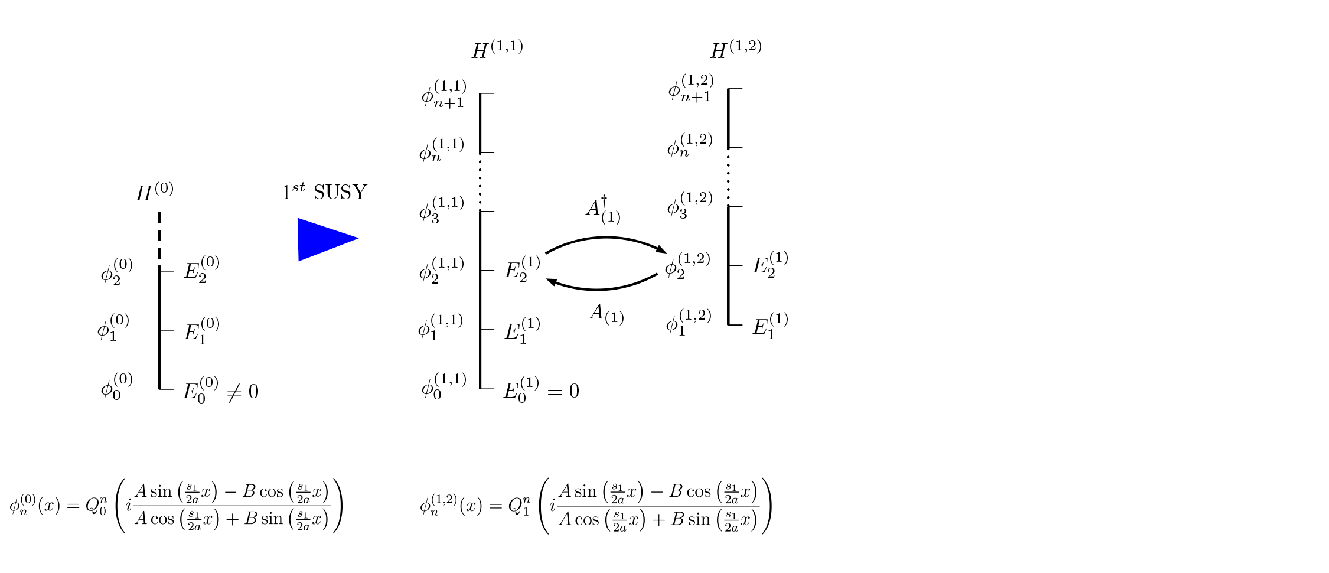
\includegraphics[width=\textwidth]{1SUSY.pdf}
			\end{figure}}
			\only<3->{\begin{figure}
					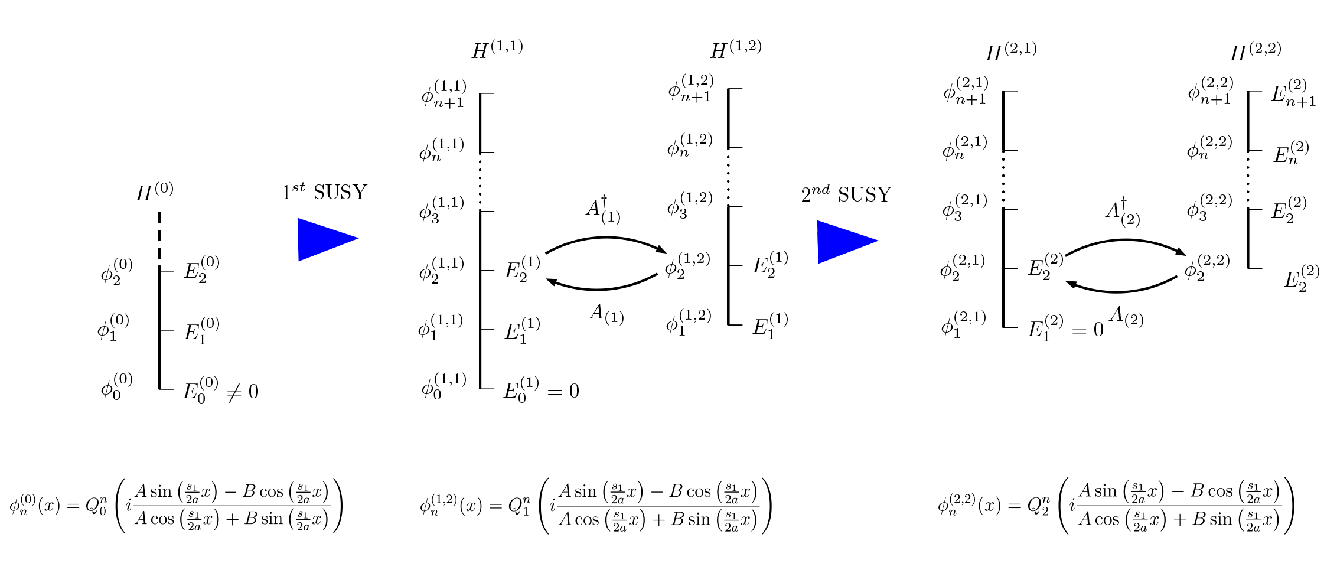
\includegraphics[width=\textwidth]{2SUSY.pdf}
			\end{figure}}
		\end{block}
		
		\uncover<4>{	\begin{alertblock}{}
				
				\begin{equation}
					\ell	\text{-ésima transformada:}\quad 	\phi^{(\ell,2)}_n(x)=Q^{n}_{\ell}\left(i\frac{A\sin\left(\frac{s_0}{2a}x\right)-B\cos\left(\frac{s_0}{2a}x\right)}{A\cos\left(\frac{s_0}{2a}x\right)+B\sin\left(\frac{s_0}{2a}x\right)} \right)\,.
				\end{equation}
		\end{alertblock}}
	\end{frame}
	
	\begin{frame}{Transformadas SUSY de las extensiones $m_2=m_3=0$}
	\only<1,2>{	\begin{block}{Clasificación de las extensiones}
			Ahora nos centraremos en el caso preferido: $m_2=m_3=0$ debido a la simplicidad de las funciones implicadas:
			\begin{columns}
				
				\begin{column}{0.3\textwidth}  %%<--- here
					\begin{block}{}
						\begin{center}
							\includegraphics[width=1\textwidth]{regionnegativas.pdf}
						\end{center}
					\end{block}
				\end{column}
				\begin{column}{0.6\textwidth}
					\begin{table}[]
						\centering
						\begin{tabular}{|c|c|c|}
							\toprule
							\textbf{Región}	& \textbf{Estado fundamental}	   & \textbf{1$^\text{os}$ niveles}  \\
							\midrule
					
						a)		& (-) y par		    &    (-,+,+,+,\dots)  \\
						b) 		& (-) e impar	  & (-,+,+,+,\dots)    \\
						c)                         &  (-) y par     & (-,-,+,+,\dots)  \\
						d)   &  (-) e impar    &   (-,-,+,+,\dots)  \\ 
						e)   &  (+) & (+,+,+,+,\dots)  \\
						b) $\cap$ d)   & (-) e impar   &   (-,0,+,+, \dots) \\
						a) $\cap$ c)   & (-) y par   &  (-,0,+,+, \dots) \\
						e) $\cap$ b)   & (0) par   &  (0,+,+,+, \dots) \\
						e) $\cap$  a)   & (0) impar   &   (0,+,+,+, \dots) \\
						Linea roja     & (-) degenerado    &  (-,-,+,+,\dots) \\
						Punto rojo&  (0) degenerado   &  (0,0,+,+,\dots) \\
						
							\bottomrule
						\end{tabular}
						
					\end{table}
				\end{column}
				
			\end{columns}
		\end{block}
	
}
\only<3>{	\begin{block}{Clasificación de las extensiones}
		Ahora nos centraremos en el caso preferido: $m_2=m_3=0$ debido a la simplicidad de las funciones implicadas:
		\begin{columns}
			
			\begin{column}{0.3\textwidth}  %%<--- here
				\begin{block}{}
					\begin{center}
						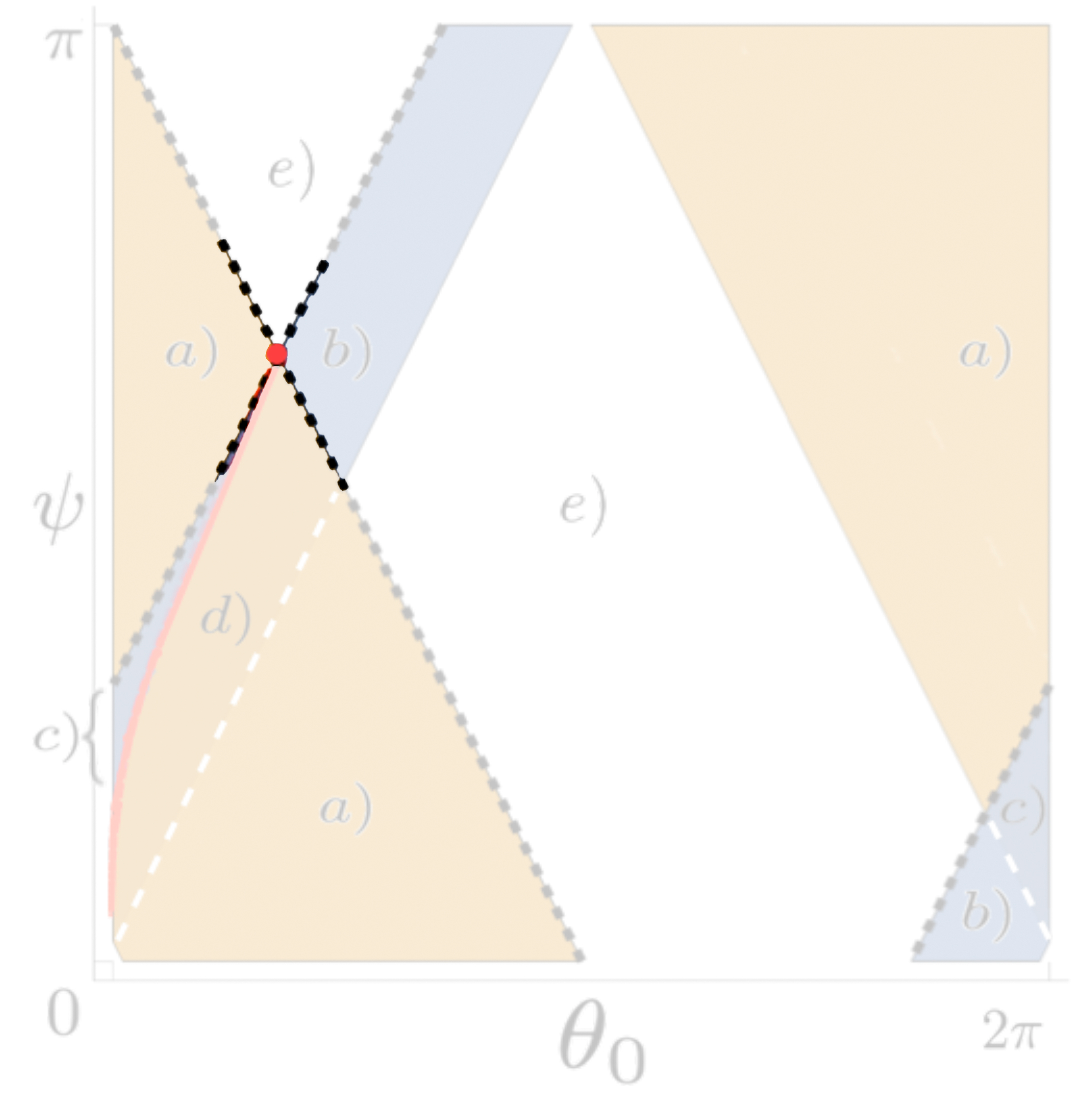
\includegraphics[width=1\textwidth]{regionnegativaspunto.pdf}
					\end{center}
				\end{block}
			\end{column}
			\begin{column}{0.6\textwidth}
				\begin{table}[]
					\centering
					\begin{tabular}{|c|c|c|}
						\toprule
						\textbf{Región}	& \textbf{Estado fundamental}	   & \textbf{1$^\text{os}$ niveles}  \\
						\midrule
					 \uncover<2>{a)} & \uncover<2>{(-) y par} & \uncover<2>{(-,+,+,+,\dots)} \\
					\uncover<2>{b)} & \uncover<2>{(-) e impar} & \uncover<2>{(-,+,+,+,\dots)} \\
					\uncover<2>{c)} & \uncover<2>{(-) e impar} & \uncover<2>{(-,-,+,+,\dots)} \\
					\uncover<2>{d)} & \uncover<2>{(-) e impar} & \uncover<2>{(-,-,+,+,\dots)} \\
					\uncover<2>{e)} & \uncover<2>{(+)} & \uncover<2>{(+,+,+,+,\dots)} \\
					\uncover<2>{b) $\cap$ d)} & \uncover<2>{(-) e impar} & \uncover<2>{(-,0,+,+, \dots)} \\
					\uncover<2>{a) $\cap$ c)} & \uncover<2>{(-) y par} & \uncover<2>{(-,0,+,+, \dots)} \\
					\uncover<2>{e) $\cap$ b)} & \uncover<2>{(0) par} & \uncover<2>{(0,+,+,+, \dots)} \\
					\uncover<2>{e) $\cap$ a)} & \uncover<2>{(0) impar} & \uncover<2>{(0,+,+,+, \dots)} \\
					\uncover<2>{Línea roja} & \uncover<2>{(-) degenerado} & \uncover<2>{(-,-,+,+,\dots)} \\
				\textcolor{	red}{Punto rojo} & \textcolor{	red}{(0) degenerado} & \textcolor{	red}{(0,0,+,+,\dots)} \\
			
						\bottomrule
					\end{tabular}
					
				\end{table}
			\end{column}
			
		\end{columns}
	\end{block}
	
}
	\end{frame}
	
	
	\begin{frame}{Transformada SUSY-C  de $\{0,0\}$  con degeneración (punto rojo)}
		\begin{block}{Funciones y niveles de energía}
			
			\begin{gather*}
				\left\{\phi_n(x)\right\}_{n=0}^\infty = \left\{1,x,\cos\left(\frac{s_2x}{2a}\right),\sin\left(\frac{s_3x}{2a}\right),\cos\left(\frac{s_4x}{2a}\right),\dots\right\}\,,\\[0.5ex]
				\left\{E_n\right\}_{n=0}^\infty = \left\{0,0,\left(\frac{s_2}{2a}\right)^2,\left(\frac{s_3}{2a}\right)^2,\left(\frac{s_4}{2a}\right)^2,\dots\right\}\,,
			\end{gather*}
		
		\end{block}
	\only<1,2>{		\begin{block}{}
				\begin{figure}
			\includegraphics[width=0.6\textwidth]{nulldeg.pdf}
				\end{figure}
		\end{block}	}
		\only<3->{
			\begin{block}{Función semilla}
				Una transformada ordinaria da lugar a: o bien a un potencial nulo o a uno  con singularidad. Una transformada de segundo orden ordinaria da lugar a un término constante.
				\begin{equation*}
					\mathcal{W}(\phi^{(0)}_0,\phi^{(0)}_1)=\text{cte.}
				\end{equation*}
			\end{block}
		\uncover<4>{
			\begin{alertblock}{Solución}
				Aplicar la una transformada SUSY-C con una de las dos funciones de energía nula como función semilla
		\end{alertblock}}
		}
	\end{frame} 
	\begin{frame}[t]{Transformada SUSY-C  de $\{0,0\}$  con degeneración (punto rojo)}
		
		\begin{columns}
			\begin{column}{0.49\textwidth}
				
				\begin{block}{Función semilla par}
					\begin{equation*}
						\phi_0^{(0)}=1
					\end{equation*}
				\end{block}
				\begin{block}{Potencial confluente}
					\begin{equation*}
						V_0^{(2,2)}(x)=\frac{2}{(x-x_0)^2}
					\end{equation*}
				\end{block}
				
			\only<1,2>{	\begin{block}{}
							\begin{figure}
								\includegraphics[width=\textwidth]{SUSYCeNulldeg}
								\caption{ SUSY-C con el nivel par}
							\end{figure}
				\end{block}}
				\only<3>{		\begin{alertblock}{Ecuación obtenida}
						\centering
					La nueva ecuación de Schrödinger, bajo un cambio de variable, viene descrita por una \alert<3>{ecuación de Bessel}
				\end{alertblock}}
			\end{column}\hfill
			\begin{column}{0.49\textwidth}
				\begin{block}{Función semilla impar}
					\begin{equation*}
						\phi_1^{(0)}=x
					\end{equation*}
				\end{block}
				\begin{block}{Potencial confluente}
					\begin{equation*}
						V_1^{(2,2)}(x)=6\frac{x^4+2 x x_0^3}{\left(x^3-x_0^3\right)^2}
					\end{equation*}
				\end{block}
			\only<1,2>{	\begin{block}{}
							
							\begin{figure}
								\includegraphics[width=\textwidth]{SUSYCoNulldeg}
								\caption{ SUSY-C con el nivel impar}
							\end{figure}
				\end{block}}
				\only<3>{	\begin{alertblock}{Ecuación obtenida}
						\centering
La nueva ecuación de Schrödinger, bajo un cambio de variable, viene descrita por una \alert<3>{ecuación fuchsiana de 5 puntos.}
				\end{alertblock}}
			\end{column}
		\end{columns}
		
	\end{frame} 
	

	
	\section[Capítulo 4]{Capítulo 4: Transformadas supersimétricas del potencial Rosen-Morse II}
		\begin{frame}{Capítulo 4: Transformadas supersimétricas del potencial Rosen-Morse II}
		\tableofcontents[currentsection]
	\end{frame}

	
	\begin{frame}[t]{El potencial Rosen Morse II}
		\begin{block}{}
			El potencial Rosen-Morse II: \begin{equation}
				V_\lambda(x)=\only<1,4->{ -\left(\lambda^2-\frac{1}{4}\right) \operatorname{sech}^2 x}\only<2,3>{\underset{\text{Pöschl-Teller}}{\textcolor{red}{\boxed{-\left(\lambda^2-\frac{1}{4}\right) \operatorname{sech}^2 x }}}} \only<1,3->{ +2\beta\operatorname{tanh} x}\only<2,3>{\underset{\text{Término asimétrico.}}{\textcolor{blue}{\boxed{+2\beta\operatorname{tanh} x\phantom{\left(\frac{1}{1}\right) }}}}}
			\end{equation}
		\end{block}
		
		\only<3>{
		{	\setbeamercolor{block title}{bg=white,fg=black}
			\begin{block}{}
				\begin{figure}
					\centering
					\animategraphics[width=7cm,autoplay]{2}{potencial/potencial-}{1}{40}
				\end{figure}
				\end{block}}}
		\only<4->{\vspace{2 cm}\begin{block}{Propiedades}
				\begin{itemize}
					\item<5-> Tomar $\beta\to-\beta\equiv x\to-x$, por lo que consideramos \alert<5>{$\beta>0$}.
					\item<6-> $V_\lambda$ es invariante bajo \alert<6>{$\lambda\to -\lambda$}.
					\item<7-> $V_\lambda$ es \alert<7>{invariante de forma}
								\end{itemize}
		\end{block}}
	\end{frame}
	\begin{frame}{Polos de la matriz $S$}
		\begin{block}{}
			Dos series de polos:
			\begin{subequations}
				\begin{equation}
					\frac{1}{2}-\lambda-i\frac{\alert<2>{k}}{2}-i\frac{\alert<2>{k'}}{2}=-n_1,\quad n_1\in \mathbb{N} \label{con1}
				\end{equation}
				\begin{equation}
					\frac{1}{2}+\lambda-i\frac{\alert<2>{k}}{2}-i\frac{\alert<2>{k'}}{2}=-n_2,\quad n_2\in \mathbb{N} \label{con2}
				\end{equation}
			\end{subequations}
		\end{block}
		
		\only<2>{	\begin{block}{}
				Donde \alert<2>{$k,k'$} son los momentos por la 'izquierda' y por la 'derecha', respectivamente, con dependencia en la energía:
				\begin{equation}
					\alert<2>{k}=\sqrt{E+2\beta},\quad     \alert<2>{k'}=\sqrt{E-2\beta}.
				\end{equation}
				Resolviendo las ecuaciones, obtenemos las siguientes expresiones para momentos y energía, para cada una de las dos condiciones de polo.
		\end{block}}
		\end{frame}
		\begin{frame}{Espectro y momentos}
	
		\setcounter{equation}{21}
	\begin{block}{Condición 1 \eqref{con1}}
					\begin{equation}
						E_{\lambda,n}=-\left(\lambda-1/2-n\right)^2-\frac{\beta^2}{\left(\lambda-1/2-n\right)^2}\tag{22a}
					\end{equation}
					\begin{equation}
						k_{\lambda,n}=\alert<3>{i}\left(\left(\lambda-1/2-n\right)+\frac{\beta}{\lambda-1/2-n}\right)\tag{23a}
					\end{equation}
					\begin{equation}
						k'_{\lambda,n}=\alert<3>{i}\left(\left(\lambda-1/2-n\right)-\frac{\beta}{\lambda-1/2-n}\right)\tag{24a}
					\end{equation}
			\end{block}
			\uncover<2->{\begin{block}{Condición 2 \eqref{con2}}
				Mismas expresiones, pero tomando \alert<2>{$\lambda\to-\lambda$}
			\end{block}}
			\uncover<3>{\begin{alertblock}{}
					Como los momentos son puramente imaginarios, se da la siguiente relación:
					
					\begin{equation*}
						\boxed{ \operatorname{Im} k_{\pm \lambda,n}=-i\,  k_{\pm \lambda,n}}
					\end{equation*}
		\end{alertblock}}
		
	\end{frame}
	\begin{frame}{Funciones de onda}
		\setcounter{equation}{24}
	
		\begin{block}{Condición 1 \eqref{con1}}
			\begin{equation}
				\phi_{\lambda,n}=M_{\lambda,n}e^{-\frac{\beta}{\lambda+1/2+n}x}\,\operatorname{sech}^{-\lambda-1/2-n}(x) \alert<1,4>{P^{(-ik_{\lambda,n},\, -ik'_{\lambda,n})}_n(\tanh x)},
			\end{equation}
			\vspace{0.5 cm}
			\begin{equation}
					\begin{split}
						\psi_{\lambda,n}= \frac{e^{-\frac{\beta}{\lambda+1/2+n}x}}{\operatorname{cosh}^{\lambda-1/2-n}(x)} \,\alert<2>{_2F_1}\left(\begin{matrix}n+1,\,n+2 \lambda +1\\[2ex] n+\lambda -\frac{ \beta }{\lambda+1/2+n}+\frac{3}{2}\end{matrix}; \frac{1+\tanh x}{2}\right).
					\end{split}
				\end{equation}
			
		\end{block}
		\uncover<3->{		\begin{block}{Condición 2 \eqref{con2}}
				Las mismas expresiones, pero tomando \alert<3>{$\lambda\to -\lambda$}
			\end{block} 
		}
		\uncover<4->{	\begin{alertblock}{}
				Las funciones con polinomios de Jacobi con argumento $\tanh x$ son $L^2(\mathbb{R})$  para valores positivos de sus parámetros $\implies -i k,-ik'>0$ 
		\end{alertblock}}
	\end{frame}
	
	\begin{frame}{Clasificación de los polos}
	
		\only<1>{{\setbeamercolor{block title}{bg=white,fg=black}	\begin{block}{}
			
				\begin{figure}
					\centering
					\includegraphics[width=0.9\textwidth]{plotkn1.pdf}
					\caption{Signo de la parte imaginaria de los momentos $\lambda>1/2+\sqrt{\beta}$}
					\label{fig:enter-label}
				\end{figure}
		\end{block}}}
		\only<2>{{\setbeamercolor{block title}{bg=white,fg=black}\begin{block}{}
				\begin{figure}
					\centering
					\includegraphics[width=0.7\textwidth]{plotkn2.pdf}
					\caption{Signo de la parte imaginaria de los momentos $\lambda>1/2+\sqrt{\beta}$}
					\label{fig:enter-label}
				\end{figure}
		\end{block}}}
		\only<3>{{\setbeamercolor{block title}{bg=white,fg=black}\begin{block}{}
				\begin{figure}
					\centering
					\includegraphics[width=0.7\textwidth]{plotkn3.pdf}
					\caption{Signo de la parte imaginaria de los momentos $\lambda>1/2+\sqrt{\beta}$}
					\label{fig:enter-label}
				\end{figure}
		\end{block}}}
		\only<4->{\setbeamercolor{block title}{bg=white,fg=black}{\begin{block}{}
				\begin{figure}
					\centering
					\includegraphics[width=0.7\textwidth]{plotkn4.pdf}
					\caption{Signo de la parte imaginaria de los momentos $\lambda>1/2+\sqrt{\beta}$}
					\label{fig:enter-label}
				\end{figure}
		\end{block}}}
	

		\visible<2->{	\begin{block}{} En función del signo de la dupla $(k,k')$ tendremos 3 tipos de polo:
		\begin{itemize}
		\item \visible<2->{\textcolor{red}{Polos ligados:} Aquellos con $\operatorname{Im}k$, $\operatorname{Im}k'>0$ }
		
		\item \visible<3->{\textcolor{darkgreen}{Polos redundantes:} Aquellos con $\operatorname{Im}k\cdot \operatorname{Im}k'<0$ }
		\item \visible<4->{\textcolor{blue}{Polos anti-ligados:} Aquellos con $\operatorname{Im}k$, $\operatorname{Im}k'<0$ }	\end{itemize}
	\end{block}}

	
	\end{frame}\begin{frame}{Clasificación de los niveles de energía}
		\begin{columns}
			\begin{column}[t]{0.59\textwidth}
				\begin{block}{Condición 1 \eqref{con1}}
					\begin{itemize}
						\item \only<1->{\textcolor{red}{Estados ligados:} $n\in \left[0,\lfloor\lambda-1/2-\sqrt{\beta}\rfloor\right]$}
						\item \only<3->{ \textcolor{darkgreen}{Estados redundantes:} Hay $\lfloor2\sqrt{\beta}\rfloor$}
						\item \only<5->{\textcolor{blue}{Estados anti-ligados:} $n\geq \lfloor\lambda-1/2+\sqrt{\beta}\rfloor$}
					\end{itemize}
				\end{block}
			\end{column}       \begin{column}[t]{0.39\textwidth}
				\only<5->{ \begin{block}{Condición 2 \eqref{con2}}
						\begin{center}
							Solo \textcolor{cyan}{Estados anti-ligados}
						\end{center}
				\end{block}}
			\end{column}
		\end{columns}
		\only<1-7>{\ \begin{center}\begin{minipage}{6.8 cm}
					
				{\setbeamercolor{block title}{bg=white,fg=black}	\begin{block}{}
						\begin{figure}
							\centering
							\only<1>{ \includegraphics[width=.99\textwidth]{states/states1.pdf}}
							\only<2>{ \includegraphics[width=.99\textwidth]{states/states20.pdf}}
							\only<3>{ \includegraphics[width=.99\textwidth]{states/states2.pdf}}
							\only<4>{ \includegraphics[width=.99\textwidth]{states/states18.pdf}}
							\only<5>{ \includegraphics[width=.99\textwidth]{states/states3.pdf}}
							\only<6>{ \includegraphics[width=.99\textwidth]{states/states17.pdf}}
							\only<7>{\animategraphics[width=.99\textwidth,autoplay]{4}{states/states}{3}{16}}
							
						\end{figure}
					\end{block}}
		\end{minipage}\end{center}}
		\only<8->{ 
			\begin{block}{Soluciones sin nodos (Nodeless)}
				\begin{enumerate}
					\item<9-> Tipo I $\phi^{I}_{\lambda,n}$: \visible<10->{\textcolor{darkgreen}{ Estados redundantes $\phi_{\lambda,n}$} para $(\lambda-1/2)\lambda<n<\beta$.}
					\item<9->  Tipo II $\phi^{II}_{\lambda,n}$: \visible<11->{\textcolor{darkgreen}{ Estados redundantes $\phi_{\lambda,n}$} para $-(\lambda-1/2)\lambda<n<\beta$}
					\item<9-> Tipo III $\phi^{III}_{\lambda,n}$: \visible<12->{\textcolor{cyan}{Estados Anti-ligados $\phi_{-\lambda,n}$} para $n=2m,\quad m\in \mathbb{Z}$}
				\end{enumerate}
				
			\end{block}}
		
	\end{frame}
	
	
	\begin{frame}{Transformadas SUSY del potencial Rosen-Morse II}
		\begin{block}{}
			Ya que el potencial es invariante de forma, una transformada SUSY ordinaria solo alterará sus  parámetros, pero no su forma funcional.
			\begin{equation*}
				H_\lambda \xrightarrow{ \substack{\text{SUSY con} \\ \phi_{\lambda,0}} }  \visible<2->{ H_{\lambda-1} \xrightarrow{ \substack{\text{SUSY con} \\ \phi_{\lambda-1,0}} }}   \visible<3->{H_{\lambda-2} \xrightarrow{ \substack{\text{SUSY con} \\ \phi_{\lambda-2,0}} } \dots}
			\end{equation*}
		\end{block}
	{	\setbeamercolor{block title}{bg=white,fg=black}	\begin{block}{}
			\only<1->{  \begin{figure}
					\centering
					\only<1->{ \begin{subfigure}[b]{0.33\textwidth}
							\centering
							\includegraphics[width=\textwidth]{si1}
					\end{subfigure}}
					\visible<2->{\begin{subfigure}[b]{0.3\textwidth}
							\centering
							\includegraphics[width=\textwidth]{si2}
					\end{subfigure}}
					\visible<3->{  \begin{subfigure}[b]{0.33\textwidth}
							\centering
							\includegraphics[width=\textwidth]{si3}
					\end{subfigure}}
			\end{figure}}
			
	\end{block}}
		\visible<4->{
			\begin{alertblock}{}
			Al ser \alert<4>{invariante de forma}, las transformadas ordinarias no alteran la dependencia funcional del potencial.
			\end{alertblock}
		}  
	\end{frame}
	\begin{frame}{SUSY con un estado redundante como función semilla}
		
		
		\begin{block}{}
			Utilizando los estados sin ceros de tipo I y tipo II .\\
			
			Ejemplo: \alert<2>{$\phi_{\text{\text{5.4}},4}$} pertenece a un estado redundante para \alert<2>{$\lambda=\text{5.4},\, \beta=4$}, siendo una \alert<2>{función nodeless de tipo I}.
			\end{block}
			
		{\setbeamercolor{block title}{bg=white,fg=black}\begin{block}{}
	
			\begin{figure}
				\centering
				\includegraphics[width=1\textwidth]{4a4.pdf}
				\caption{SUSY rota utilizando un estado redundante como función semilla}
				
			\end{figure}
		\end{block}}
	\end{frame} 
	\begin{frame}{SUSY con un estado anti-ligado como función semilla}
		\begin{block}{}
			Utilizando una de las funciones sin nodos tipo III, podemos obtener una SUSY de tipo II, en la que se agrega un nivel.\\
			
	Ejemplo: \alert<2>{$\phi_{-\text{2.4},2}$} es una función anti-ligada para \alert<2>{ $\lambda=\text{2.4},\, \beta=1$}, siendo una \alert<2>{función nodeless de tipo III}.
		\end{block}
		
	{\setbeamercolor{block title}{bg=white,fg=black}	\begin{block}{}
			\begin{figure}
				\centering
				\includegraphics[width=1\textwidth]{1a2.pdf}
				\caption{SUSY de tipo II a partir de un estado anti-ligado sin nodos}
				
			\end{figure}	
\end{block}}
	\end{frame} 
	\begin{frame}[t]{Equivalencia entre poner/quitar niveles}
		\begin{block}{}
			Consideremos \alert<1>{$\lambda=\text{5.4}$ y $\beta=1$}, una SUSY de segundo orden (no ordinaria) utilizando los dos primeros estados excitados como función semilla.
		\end{block} 
	
	\visible<2->{
		{\setbeamercolor{block title}{bg=white,fg=black}	\begin{block}{}
				\begin{figure}
					\centering
					\only<2>{\includegraphics[width=1\textwidth]{4a2.pdf}}
					\only<2>{\caption{Transformación que elimina dos niveles.}}
					\only<3->{\includegraphics[width=1\textwidth]{equiv.pdf}}
					\only<3->{\caption{Equivalencia entre las dos últimas transformaciones.}}
				\end{figure}
	\end{block}}}
		\visible<4->{\begin{alertblock}{}
				\begin{itemize}
					\item Existe una relación entre \alert<5>{eliminar dos niveles en $\lambda=\text{5.4}$} y crear un nivel el \alert<5>{potencial con $\lambda=\text{2.4}$}. 
					\item En la publicación correspondiente a este artículo aparece demostración para \alert<6>{$\lambda$ arbitraria}, y \alert<6>{eliminar $N$ niveles }.
				\end{itemize}
		\end{alertblock}}
	\end{frame}
	\section[Conclusiones]{Conclusiones}
	
	\begin{frame}{Conclusiones.}
		\tableofcontents[currentsection]
	\end{frame}
	\begin{frame}{Conclusiones}
	\uncover<2->{	\begin{block}{Capítulos 2 y 3 (correspondientes a [1] y [2]) :}
			
			\begin{itemize}
				
				
				\item Se ha obtenido una nueva \alert<3>{clasificación de las extensiones autoadjuntas} del operador $-\partial_x^2$ restringido a un intervalo finito.
				\item  Nuevas soluciones de ecuaciones ya conocidas (\alert<4>{Bessel})  y desconocidas (\alert<4>{caso particular de una fuchsiana}).
				\item  Generalización de la \alert<5>{transformada de orden $\ell$} para una SUSY ordinaria cuando la función semilla no tiene simetría $PT$.
			\end{itemize}
	\end{block}}
	\visible<5->{	\begin{block}{En el Capítulo 4 (correspondiente a [3]):}
			
			\begin{itemize}
				\item Equivalencia entre las condiciones para los \alert<6>{momentos} con la condición de $L^2(\mathbb{R})$ de las funciones de onda dadas por \alert<6>{polinomios de Jacobi}.
				\item Se han demostrado equivalencias de \alert<7>{operadores de intercambio} recurriendo a las segundas soluciones y al formalismo de SUSY con wronskianos.
				\item Todos los tipos de  polo permiten crear  \alert<8>{todos los tipos} de SUSY.
			\end{itemize}
	\end{block}}
	\end{frame}

	\begin{frame}{Lineas de investigación abiertas}
		\begin{block}{Extensiones autoadjuntas}
			\begin{itemize}
			\item Utilizar el \alert<2>{análisis funcional} para determinar la relación entre \alert<2>{condiciones de contorno} y \alert<2>{potenciales singulares}.
				\item Aprovechar que el espectro del hamiltoniano de llegada es conocido (de valor real) para el estudio de sistemas \alert<3>{$PT-$ simétricos y potenciales complejos}.
				
			\end{itemize}
		\end{block}
	\uncover<4->{	\begin{block}{Transformadas supersimétricas}
			\begin{itemize}
				\item Estudiar sistemas de \alert<4>{más de una dimensión}. 
				\item Estudiar otros sistemas que permitan llegar a \alert<5>{soluciones particulares de otras ecuaciones diferenciales}.
			\end{itemize}
	\end{block}}
	\uncover<5->{	\begin{block}{Potencial Rosen-Morse II}
			\begin{itemize}
				\item Aprovechar los resultados de los \alert<6>{operadores de intercambio} para facilitar el cálculo de los \alert<6>{operadores escalera} de este potencial.
			\item Posibilidad de utilizar las transformadas SUSY de este potencial para mejorar su \alert<7>{descripción fenomenológica} en física molecular.
				
			\end{itemize}
	\end{block}}
	\end{frame}


	\begin{frame}

	\begin{center}
		
		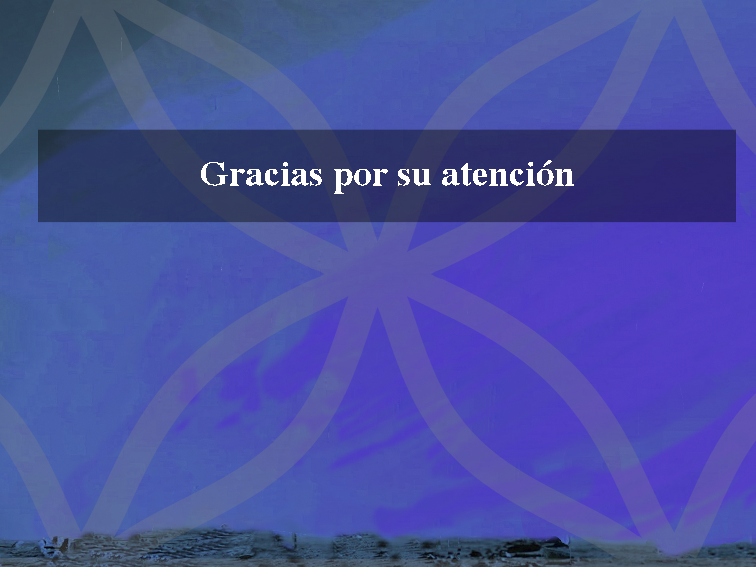
\includegraphics[width=\textwidth]{final1.pdf}
		\end{center}
	\end{frame}
	
\end{document}